\documentclass[12pt]{letter}
\usepackage{amssymb,amsmath}

\usepackage[utf8]{inputenc}
\usepackage{graphicx, graphics, epsfig}
\usepackage{epstopdf}
\usepackage{ifpdf}   
\usepackage{amsfonts}
\usepackage[english,russian]{babel}
%\usepackage[pdftex,unicode]{hyperref}
%\usepackage[noend]{algorithm}
%\usepackage[noend]{algpseudocode}
\usepackage{multicol}
\textheight=24cm
\textwidth=16cm
\oddsidemargin=0pt
\topmargin=-1.5cm
\parindent=24pt
\parskip=0pt
\tolerance=2000
\flushbottom
\def\baselinestretch{1.2} 

\author{Вишневский~Валерий~Викторович}


\begin{document}

%\thispagestyle{empty}
Имеем 2 паттерна, которые хотим соединить. Как-то зафиксировали их начала и концы.
Далее, имеем распределение расстояний на которых второй паттерн встречается после первого.
Каждая точка в этом распределении говорит, на каком расстоянии находится конец $j$-го паттерна
от начала $i$-го. У каждой реализации паттерна(тут мы пришли к дискретизации и называем конкретные
моменты времени, где паттерн имеет место быть!) существует свое правдоподобие($\alpha_i, \beta_j $).

Рассмотрим следующую сумму $k$:
\[
\begin{aligned}
k&=\sum_{i=1}^N w_ig_i(\mu,\sigma),   \\
w_i&=\alpha_i\beta_i, \\
g_i(\mu,\sigma)&=\frac{1}{\sqrt{2\pi}\sigma}exp\left(- \frac{(x_i-\mu)^2}{\sigma^2} \right) 
\end{aligned}
\]
Так же, пусть:
$$
\begin{aligned}
S(\sigma) &= \sigma\sqrt{2\pi}, \text{ площадь под гауссианой};\\
N &\text{--- количество точек в распределении};\\
N_{eff} &= \frac{\sum_{i=1}^N w_i}{\max_i{w_i}};\\
M &\text{--- размер окна}
\end{aligned}
$$
В общем примерно так:\\
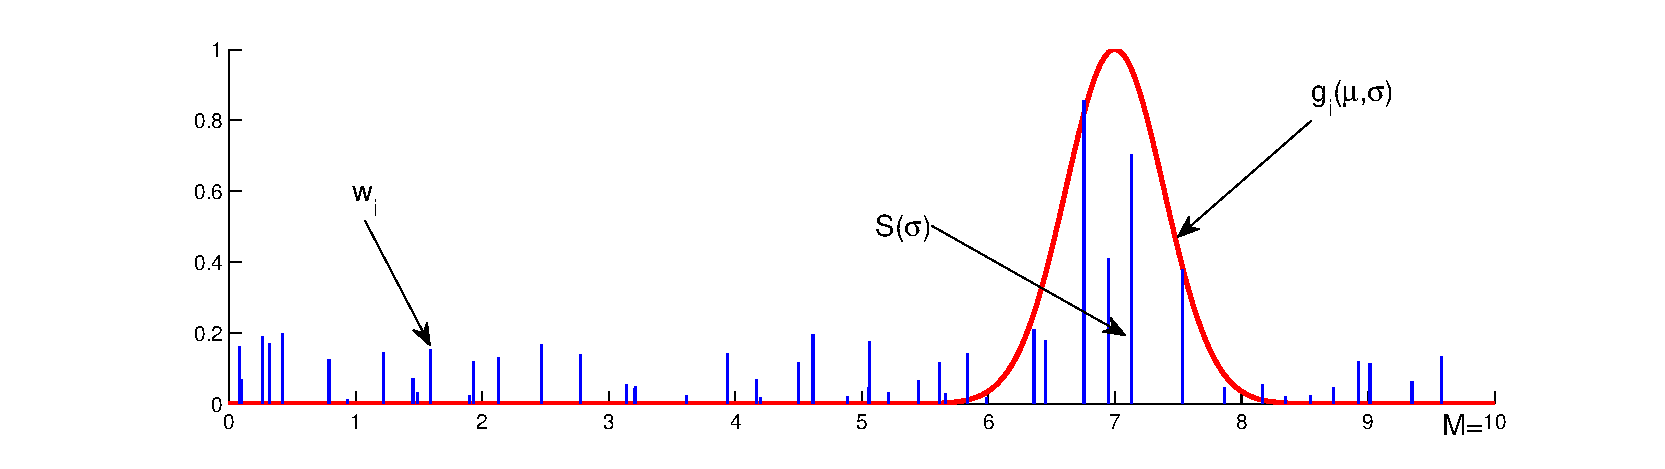
\includegraphics[width=200mm]{example.eps}
Если принять гипотезу о равномерном распределении расстояний(нулевая гипотеза~-- в данных нету никаких
закономерностей, то случайная величина k будет иметь, по ЦПТ, при $N\to\infty$ следующее распределение:
$$
\begin{aligned}\label{Norm}
k &\sim N \left( \frac SM N, \frac{(M-S)S}{M^2}N \right), \text{--- если $w_i=1$} \\
k &\sim N \left( \frac SM N~ mean({w_i}), \frac{(M-S)S}{M^2}N disp(w_i)  \right), \text{--- пытаемся учесть $w_i$~~~~(1) } 
\end{aligned}
$$
Вот что получается на практике, если $w_i$ брать из равномерного распределения(более мы ничего не можем о нем сказать). 
Надо отметить, что при  $ N < 50 $ мат ожидание бывает слегка сдвинуто. Следующие графики представлены для значений $N$ 1000 и 20 соответственно.\\
\includegraphics[width=200mm]{norm.eps}
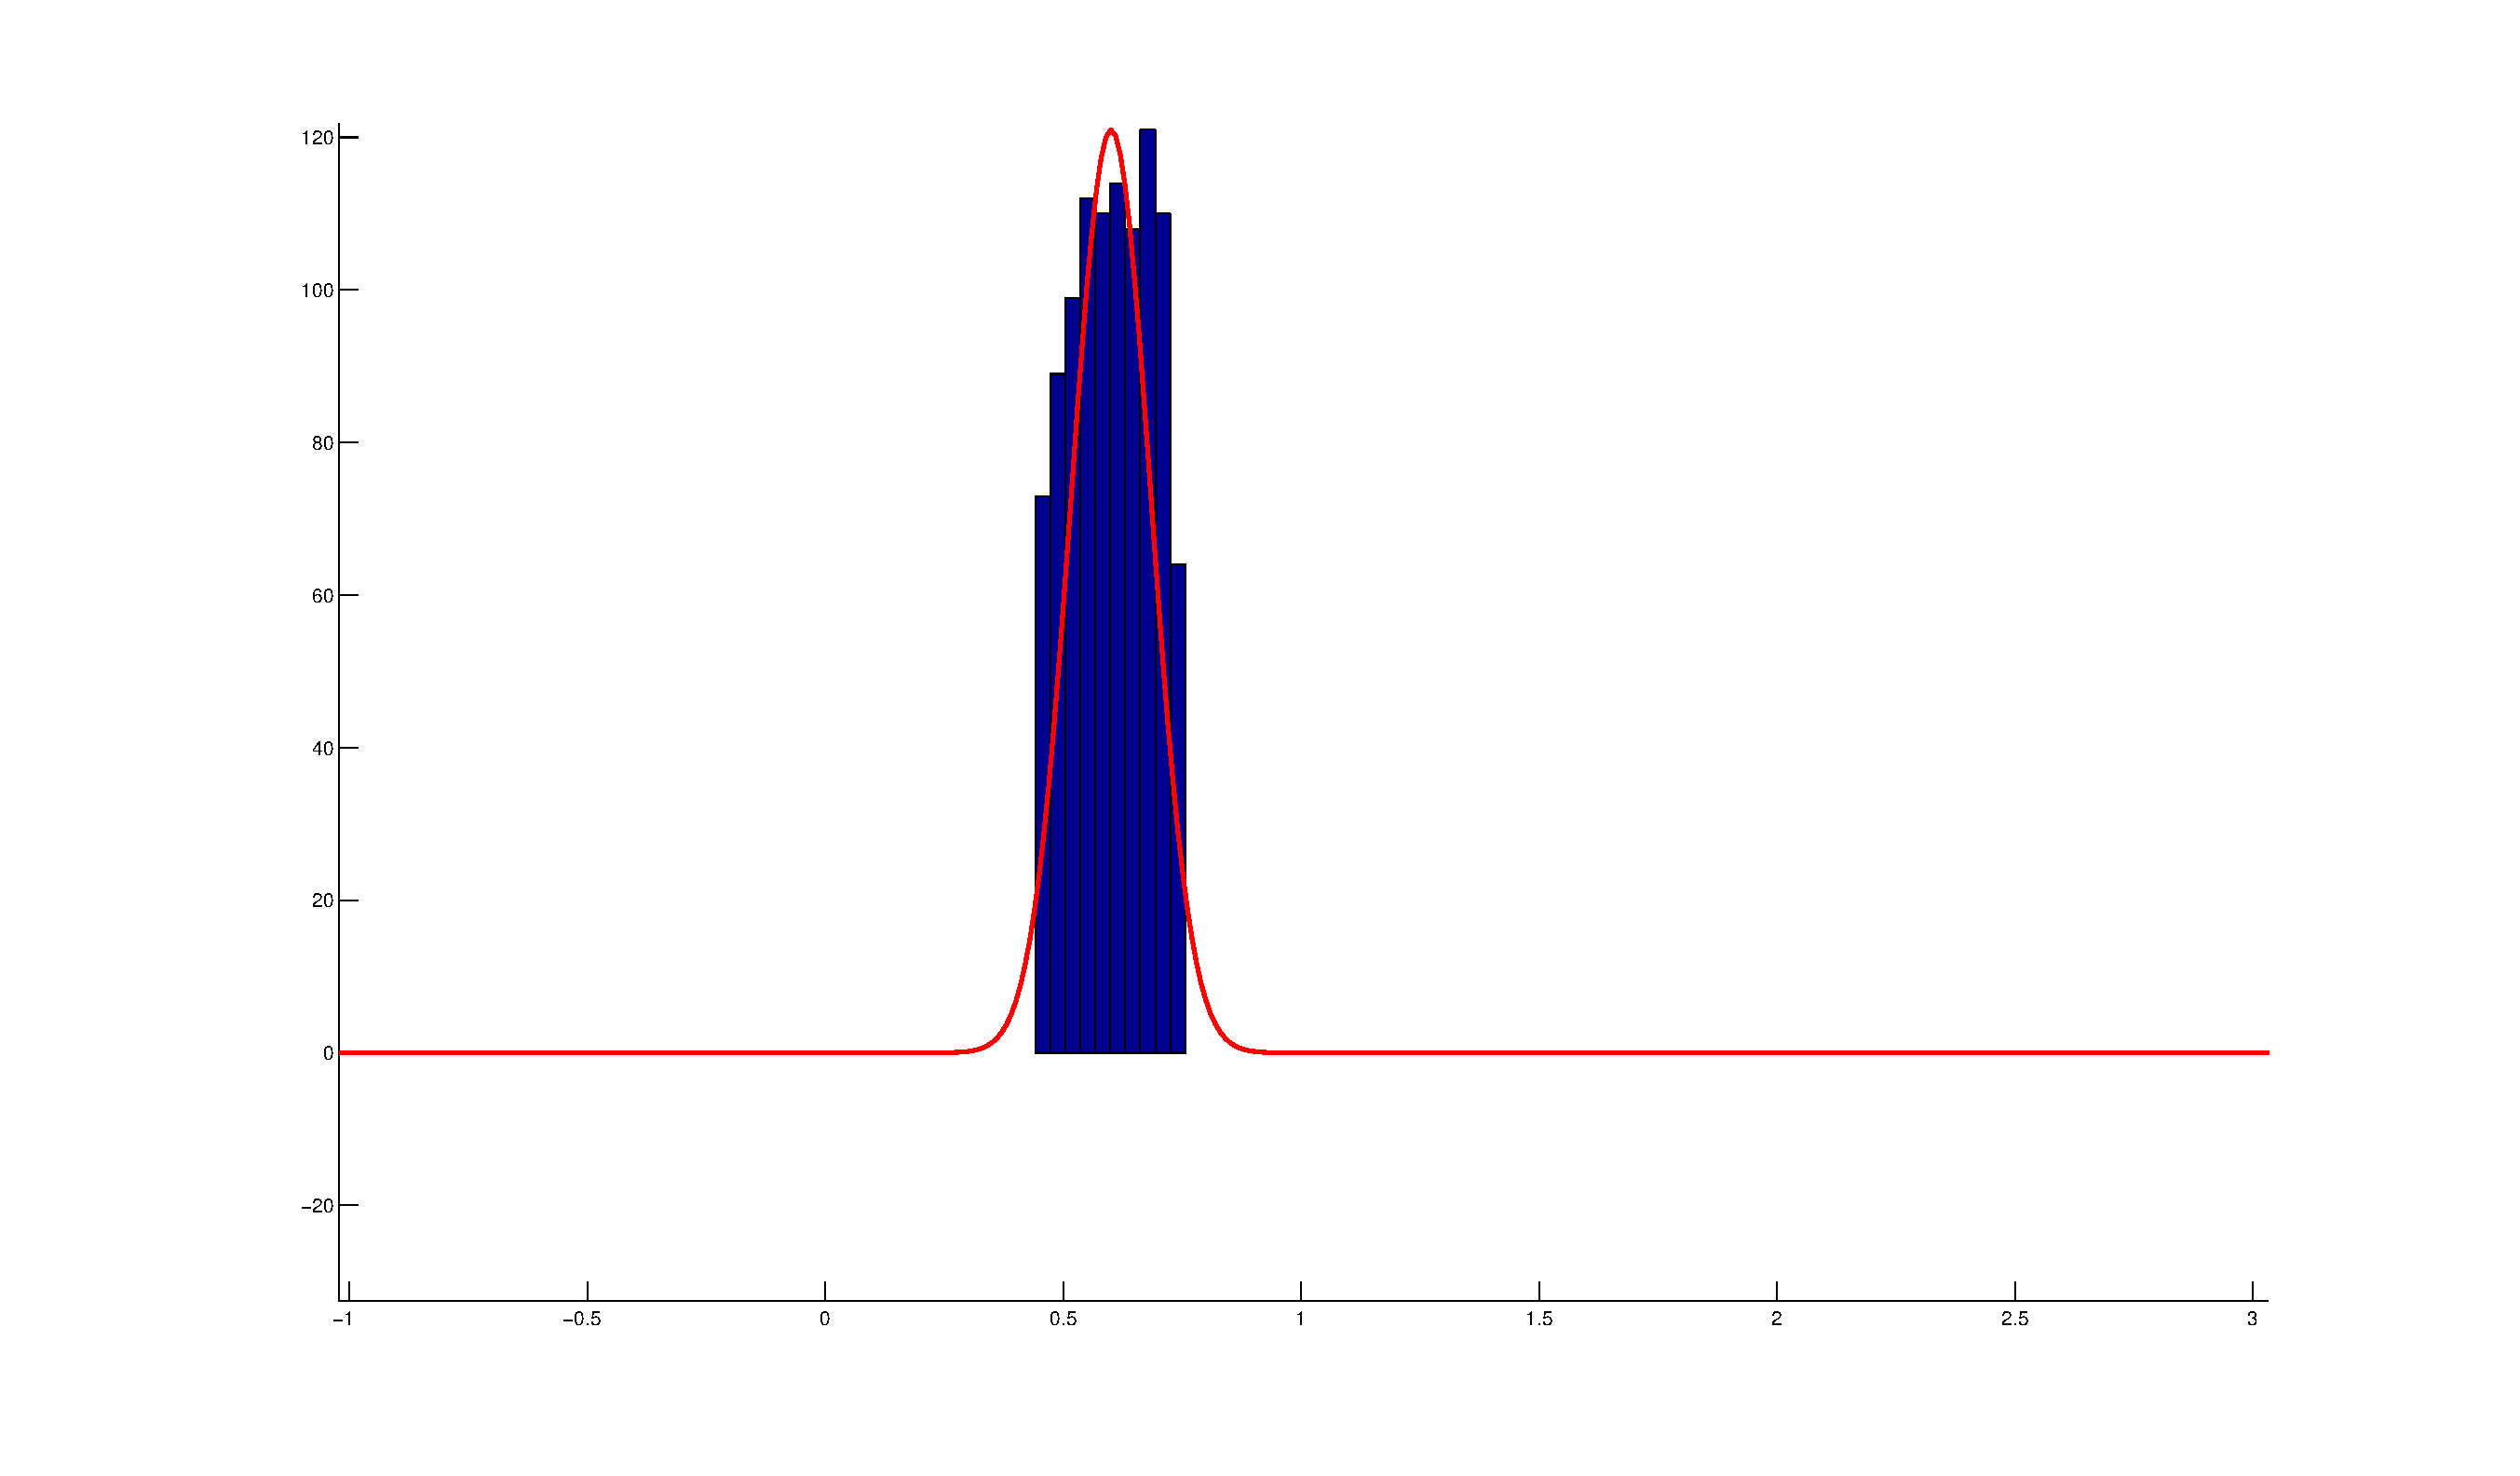
\includegraphics[width=200mm]{norm20.eps}

Теперь нужно на реальных данных вычислить значение величины $k$ и посмотреть на сколько оно было вероятно, исходя из формулы (1). 
Чем меньше вероятность данного события в случайных денных, тем больше оно похоже на паттерн. Идея, в общем, такая...\\
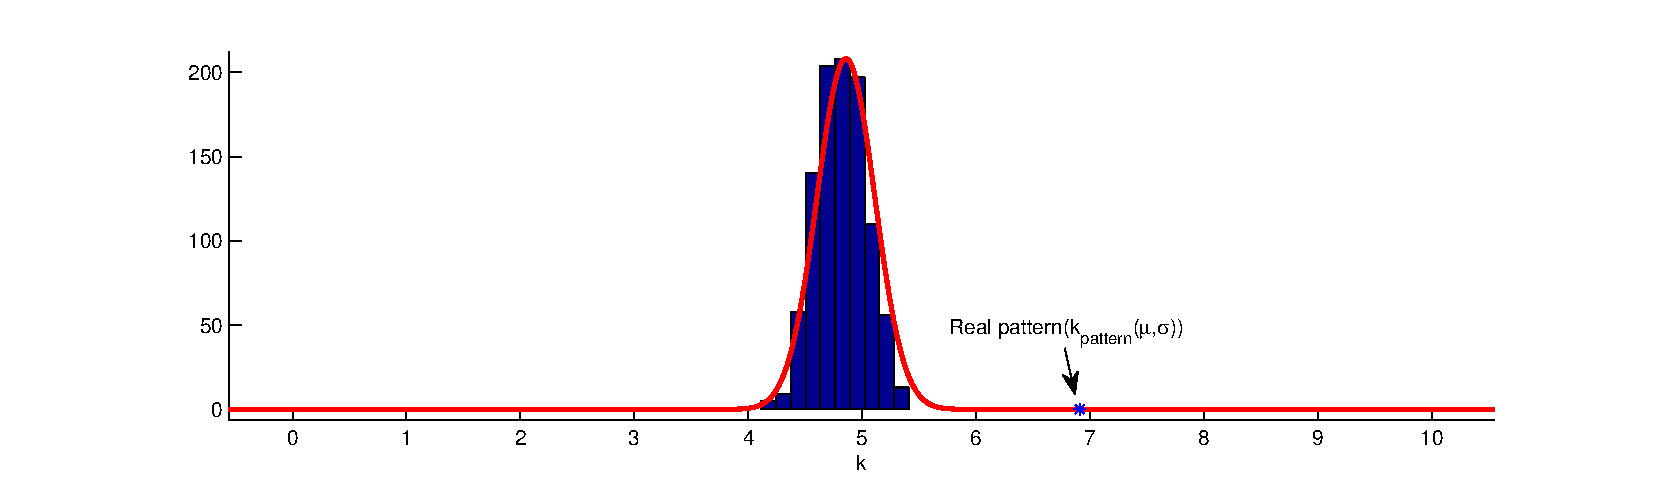
\includegraphics[width=200mm]{pattern.eps}
Таким образом, мы должны минимизировать:
$$
\left\{
\begin{aligned}
N_{\left(  \frac SM N~ mean({w_i}), \frac{(M-S)S}{M^2}N disp(w_i)  \right)}[k_{pattern}(\mu,\sigma)] \to \min_{\mu,\sigma}\\
k_{pattern}(\mu,\sigma) > \frac SM N~ mean({w_i})
\end{aligned}
\right.
$$
Здесь второе условие использовано для того что бы показать, что нам нужен именно правый <<хвост>> гауссианы.

%\includegraphics[width=90mm]{chooseMy+Alena+Order1.eps}
%\includegraphics[width=90mm]{chooseMy+Order0+Katya.eps}
%\includegraphics[width=90mm]{chooseMy+Order1+Katya.eps}
%\includegraphics[width=90mm]{chooseMy+Alena+Katya.eps}
%\includegraphics[width=90mm]{calcMy+Alena+Order0.eps}
%\includegraphics[width=90mm]{calcMy+Alena+Order1.eps}
%\includegraphics[width=90mm]{calcMy+Order0+Katya.eps}
%\includegraphics[width=90mm]{calcMy+Order1+Katya.eps}
%\includegraphics[width=90mm]{calcMy+Alena+Katya.eps}



\newpage
\end{document}
